% Created 2023-10-01 Sun 08:53
% Intended LaTeX compiler: pdflatex
\documentclass[11pt]{article}
\synctex=1
\usepackage[utf8]{inputenc}
\usepackage[T1]{fontenc}
\usepackage{graphicx}
\usepackage{longtable}
\usepackage{wrapfig}
\usepackage{rotating}
\usepackage[normalem]{ulem}
\usepackage{amsmath}
\usepackage{amssymb}
\usepackage{capt-of}
\usepackage{hyperref}
\usepackage[margin=1in]{geometry}
\usepackage{mathtools}
\usepackage{multirow}
\usepackage{tabularx,longtable,multirow,subfigure,caption}
\usepackage{booktabs}
\usepackage{bm}
\author{Alvaro Cea and Rafael Palacios}
\date{\today}
\title{First deliverable Report}
\hypersetup{
 pdfauthor={Alvaro Cea},
 pdftitle={First deliverable Report},
 pdfkeywords={},
 pdfsubject={},
 pdfcreator={Emacs 29.1 (Org mode 9.6.6)}, 
 pdflang={English}}
\begin{document}

\newcommand{\bs}[1]{\boldsymbol{#1}}
\newcommand{\rhoinf}{\rho}	
\newcommand{\Vinf}{U}
\newcommand{\Cl}[1]{c_{l_{#1}}}
\newcommand{\barCl}[1]{\bar{c}_{l_{#1}}}
\newcommand{\Cm}[1]{c_{m_{#1}}}
\newcommand{\barCm}[1]{\bar{c}_{m_{#1}}}
\newcommand{\AIC}{\bs{\mathcal{A}}}


\maketitle
\tableofcontents


\section{Introduction}
\label{sec:orgad08129}
This work continues the development of an alternative approach \cite{CEA2021,CEA2023} to study the
geometrically nonlinear effects of already existing (linear) industrial-scale aeroelastic models.
The method blends the efficiency and accuracy of geometrically-exact 1D descriptions for prob-
lems involving slender components, with the precision of condensation techniques in preserving
the full 3D characteristics. It seamlessly integrates with standard linear aeroelastic analysis
based on finite element solvers and compressible potential aerodynamics. The novelty is that
the geometric-nonlinearity is included by considering information about the nodal coordinates,
which are not tracked in linear modal analysis. The information for the geometric nonlineari-
ties is introduced from the geometric layout of the structure which results in coupling between
modes. This is facilitated by Hodges’ intrinsic equations [216]: by construction, the sectional
velocities and internal forces have local influence regardless of large rigid-body rotations, and
this does not need updating of the local mass and stiffness properties from the initial config-
uration. This feature permits the addition of geometrically-nonlinear effects to a predefined
complex linear model.

This feature permits the addition of geometrically-nonlinear effects to a predefined
complex linear model. In addition, only quadratic terms of the main variables are needed to capture nonlinear effects. Our concern is a problem of relatively high geometrical complexity
for which a (linear) finite-element model (FEM) already exists, not necessarily built with beam
elements, but representing a physical domain with a dominant dimension. The goal is to seek
a computationally-efficient solution strategy that leverages on the slenderness of the domain
to characterise geometrically-nonlinear effects, while utilising the information encapsulated in
the original model –which is built, validated and refined during the design cycle of the specific
engineering asset under consideration.

The resulting solution procedure can be divided into the five stages shown in Fig.: 1) A
linear (arbitrarily complex) model with slender components is the input for the analysis. 2)
Model condensation is employed to derive a skeleton-like substructure, along the main load
path, containing the main features of the full 3D model. 3) The modes of the reduced structure
are evaluated in intrinsic variables (velocities and strains) and used as a basis of a Galerkin-
projection of the geometrically-nonlinear intrinsic beam equations. 4) The projected equations
are solved in time-domain under given forces: aerodynamic influence coefficient matrices are
obtained from DLM and a rational function approximation (RFA) is used to transform to the
time domain. 5) The intrinsic modes, the reduced order transformations, and the nonlinear 1D
solution are combined to reproduce the full 3D solution. Geometrically-nonlinear behaviour
is captured along the principal skeleton and the linear response of the cross-sections (in the
form of ribs and fuselage reinforcements) is also represented –if nonlinear deformations also
occur in the cross-sections, there is no reliable analysis other than high-fidelity solutions of the
full model. The overall procedure has been implemented in what we have named as Nonlinear
Modal Reduced Order Model (NMROM).
\begin{figure}[htbp]
\centering
\includegraphics[width=.75\linewidth]{./img/aircraft_process.pdf}
\caption{\label{fig:org4a19cf9}Solution process chart using the present approach}
\end{figure} 
%
\section{Theoretical background}
\label{sec:org068f350}

\subsection{Airframe idealisation}
\label{sec:org78ded7e}
The basis for the mechanics of solids is laid in this chapter and represents the foundation for the structural solution that incorporates geometrical nonlinear effects to already existing (linear) models in a non-intrusive manner. Firstly, the physics driving the dynamics of solid bodies are described and will serve to derive, from first principles, the nonlinear beam equations ultimately conforming the aeroelastic methodology in following chapters. A subset of (well-known) structural problems are those of linear elasticity, and reduced order modelling techniques will allow to bridge the gap between them and a nonlinear one-dimensional description  through  a mapping of modal information. Therefore the fields of 3D elasticity, reduction order modelling, and geometrically-nonlinear dynamics of slender structures are brought together in a compact formulation: the starting point is an arbitrarily complex FE model for which structural dynamic condensation techniques are employed to reduce the 3D components into nodes along all major load paths (a skeleton-like substructure), in line with current industrial practice. The resulting linear normal modes (LNMs)  are evaluated in intrinsic variables (velocities and strains) and used as a basis of a Galerkin-projection of the geometrically-nonlinear intrinsic beam equations in modal space. Thus a second  reduction is possible by selecting the size of the modal basis employed in the solution. We generalize previous formulations with a four field description (velocity, momentum, strain, and internal forces) that enables  the use of arbitrary reduction techniques and  structures with distributed inertia. The projected equations are solved in time domain and the full 3D field can be obtained as a post-processing step. \\
The workflow of the different theories presented in this chapter is shown in Fig. \ref{fig2:aircraft2NMROM}, with the starting point as the  airframe of an aircraft that we want to approximate mathematically. The fundamentals of solid mechanics are first introduced, which leads to a  nonlinear 1D approximation after a set of kinematic assumptions on one hand, and to the equations of linear elasticity on the other; discretisation of the linear equations and applying the appropriate boundary conditions produce the FE models used by organizations in the design process. They are enhanced with experimental tests to account for the missing details in mathematical process. The combination of the 1D description with a condensed version of the FE model along the main load paths allows the construction of a \emph{Nonlinear Modal Reduced Order Model} (NMROM) that combines all the theories in the figure and, as presented in the next chapters, it  serves as the core tool to attain efficient aeroelastic computations. In fact, the construction of an aeroelastic system based on this NMROM is one of the main novelties of this work. In the process, the reduction techniques presented in sec. \ref{sec:Linear Reduction Order Models in Structural Dynamics} have been explored to capture, as accurate as possible, the characteristics of the full FE model derived from linear elasticity; the solution of the intrinsic equations in modal space, sec. \ref{sec2:Geometrically nonlinear mechanics of slender structures}, and  the subsequent derivation of the relation between modal shapes and their couplings in the equations, sec. \ref{Bridging full and reduced descriptions through the modal spaces},  is a key result that allows the seamlessly incorporation of geometrically-nonlinear effects to the (condensed) linear FE models;  along the entire chapter, some light is shed into the direct relation between the 1D description and the main principles of solid mechanics, including the recovery of the 3D displacement field from the reduced nonlinear solution, presented for the first  time in sec. \ref{sec2:3d_recovery}. Therefore all subjects in Fig. \ref{fig2:aircraft2NMROM} are introduced in this chapter, except for the experimental part of model updating, which could well be part of a future development and validation with real structures. 
%
%\newpage
\begin{figure}[h!]
\centering
\includegraphics[width=0.9\textwidth]{./img/reality2NMROM2}
\caption{Fields and assumptions leading to the construction of a structural  NMROM of representative airliners.}\label{fig2:aircraft2NMROM}
\end{figure}

\subsection{Dynamic condensation of linear FE models}\label{sec:dynamic_condensation}
Model order reduction techniques aim to increase computational efficiency by reducing the size of the problem while maintaining its fundamental characteristics. In the realm of industrial applications, ROMs are very important, even when the majority of the analysis is linear, due to the need for fast simulations and the very large models that can surpass the hundreds of thousands of DoF.  Also they have been useful in experimental modal analysis, for measurement devices can only be put in a limited number of places and the complete response has to be reconstructed for validation purposes; structural vibrations and buckling, structural optimization, or damage detection are some of the applications of these techniques \cite{Qu2010}. In aircraft loads analysis, trim and stability studies, it is common practice condensing the (linear) full-FE models into the major load paths of the aircraft, to reduce the total number of DoF to a few hundreds. Herein we not only use a condensation approach to reduce the size of the model, but also to represent a structure that can be modelled as a one-dimensional domain --making use of the slenderness of high $AR$ aircraft, where the span of wetted-surfaces and the fuselage length take predominance over the other dimensions. Therefore, consider again the solid domain $\Omega$ in Sec. \ref{sec2:Deformation of bodies and conservation laws}, defining the 3D structure, and a 1D sub-domain in which the deformable curve $\Gamma$ defines an internal load path. The points conforming $\Gamma$ either belong to the 3D structure or are a weighted average of neighboring points.  Fig. \ref{fig2:structural_condensation} illustrates a typical discretisation of both 3D and 1D domains in a simplified aircraft structure. In the aerodynamic surfaces, the interpolation elements in blue relate the active nodes in the load path to the corresponding cross-sectional nodes of the 3D structure. On the other hand, the fuselage is modelled as a rigid beam, and its nodes are part of both the full and reduced models. The nodes of the condensed model, in red, represent the discretization of $\Gamma$, where the geometrically nonlinear dynamics will be described.
%
After a finite-element discretization, eq. \eqref{eq2:linear_fem} yields the linear structural dynamics equations with respect to a common inertial reference frame.  In order to obtain the condensed model, the degrees of freedom of the full model are divided into those on active (or master) nodes, located along the load path $\Gamma$, and those of the omitted (or slave) nodes. The displacement vector can therefore be reordered as, $ \pmb{u}_n= \left(\pmb{u}_a^\top \;\pmb{u}_o^\top\right)^\top$, and similarly for the LNMs of the unloaded structure $\pmb{\Phi}=[\pmb{\Phi}_a^\top \; \pmb{\Phi}_o^\top]^\top$, so that the eigenvalue problem of $\bm{K}$ and $\bm{M}$ is arranged as,
\begin{equation}
\left( \begin{bmatrix}
\bm{K}_{aa} & \bm{K}_{ao} \\ \bm{K}_{oa} & \bm{K}_{oo}
\end{bmatrix} - \omega^2\begin{bmatrix}
\bm{M}_{aa} & \bm{M}_{ao} \\ \bm{M}_{oa} & \bm{M}_{oo}
\end{bmatrix}
\right)
\begin{pmatrix}
\bm{\Phi}_a \\ \bm{\Phi}_o
\end{pmatrix} = 0
\end{equation}
A linear dependency is now assumed between the omitted and the active degrees of freedom, 
\begin{equation}\label{eq2:Toa}
\pmb{\Phi}_o =  \pmb{T}_{oa} \pmb{\Phi}_a
\end{equation}
with $\pmb{T}_{oa} \in \mathbb{R}^{o\times a}$ the transformation matrix between both sets.
The quality of the transformation is determined by its accuracy in capturing a subset of interest of the full-system LNMs, which is linked to the spatial sampling that $\pmb{\Phi}_a$ introduces on the full domain.
In general, the condensation is dependent on the frequencies and forms a nonlinear eigenvalue problem where each LNM,  with natural frequency, $\omega_j$, has one transformation matrix,
\begin{equation}\label{eq2:transformation_exact}
\pmb{T}_{oa}(\omega_j) = (\pmb{K}_{oo}-\omega^2_j \pmb{M}_{oo})^{-1}( \pmb{K}_{oa}- \omega_j^2 \pmb{M}_{oa}) \approx -(\pmb{K}_{oo}^{-1}+\omega^2_j\pmb{K}_{oo}^{-1}\pmb{M}_{oo}\pmb{K}_{oo}^{-1})(\pmb{K}_{oa}-\omega^2_j\pmb{M}_{oa})
\end{equation}
This is the so-called exact-condensation matrix, where we have also introduced Kidder's mode expansion \cite{Qu2010} (right-hand-side expression in \eqref{eq2:transformation_exact}) to avoid repeated calculation of the inverse in the first term. The first-order approximation of this equation is attained by letting $\omega_j =0$, thereby removing inertia effects. This results in a static condensation, proposed by Guyan and Irons in 1965 \cite{Guyan1965}, still one of the most popular condensation methods today, also known as Guyan reduction. Note that when the mass model consists only of lumped masses on the active degrees of freedom, $\pmb{M}_{oo} = \pmb{M}_{oa} = \pmb{0}$, Guyan reduction is the exact condensation.  It can be proved \cite{Qu2010} that this reduction technique is the zeroth order approximation to the power series expansion of the dynamic condensation.  A further approximation including the effect of distributed inertia is obtained by selecting a single natural frequency in  \eqref{eq2:transformation_exact} for all LNMs such that the terms $\pmb{M}_{oo}$ and $\pmb{M}_{oa}$ appear in the approximation and the inertia effects are included at the selected frequency. Therefore that one frequency is exactly approximated, while accuracy is gradually lost when moving away from it . After calculation of $\pmb{T}_{oa}$, the transformation from the active set and the full model is defined as $\pmb{T} =[\pmb{I}_a \; \pmb{T}_{oa}^\top]^\top$, with $\pmb{I}_a$ the identity matrix of dimension $a$. The condensed mass and stiffness matrices are obtained by equating the kinetic energy, $\mathcal{E}_k$ and the potential energy, $\mathcal{E}_p$ in the linear reduced and complete systems; if external loads are applied to the omitted nodes, equating virtual work gives the equivalent loads in the condensed model:
\begin{equation}\label{eq2:energy_condensed_matrices}
\begin{split}
\mathcal{E}_p &= \frac{1}{2}\bm{u}_n^\top\bm{K}\bm{u}_n \cong \frac{1}{2}\bm{u}_a^\top\bm{T}^\top\bm{K}\bm{T}\bm{u}_a = \frac{1}{2}\bm{u}_a^\top\bm{K}_a\bm{u}_a \\
\mathcal{E}_k &= \frac{1}{2}\dot{\bm{u}}_n^\top\bm{M}\dot{\bm{u}}_n \cong \frac{1}{2}\dot{\bm{u}}_a^\top\bm{T}^\top\bm{M}\bm{T}\dot{\bm{u}}_a = \frac{1}{2}\dot{\bm{u}}_a^\top\bm{M}_a\dot{\bm{u}}_a \\
\mathcal{W}_f &=\delta \bm{u}_n^\top \bm{F} \cong \delta \bm{u}_a^\top \bm{T}^\top \bm{F} = \delta \bm{u}_a^\top  \bm{F}_a 
\end{split}
\end{equation}
so that condensed stiffness and mass matrix are obtained as $\pmb{K}_a = \pmb{T}^\top\pmb{K}\pmb{T}$, $\pmb{M}_a = \pmb{T}^\top\pmb{M}\pmb{T}$, and the external forces $\bm{F}_a = \bm{T}^\top \bm{F}$. The LNMs in the active set are then $\pmb{K}_a\pmb{\Phi}_{aa}=\pmb{M}_a\pmb{\Lambda}_a\pmb{\Phi}_{aa}$, with $\pmb{\Lambda}_a$ the diagonal matrix of squared natural frequencies (in what follows the approximation between the mode shapes of the full FE at the condensed points, $\pmb{\Phi}_{a}$, and the shapes directly obtained from the condensed matrices is assumed equivalent, $\pmb{\Phi}_{aa} \approx \pmb{\Phi}_{a}$, and $\pmb{\Phi}_{aa}$ is just referred as $\pmb{\Phi}_{a}$  for simplicity).
Let us look into more accurate approaches than Guyan and first order dynamic condensation, such as iterative methods which refine the reduced matrices at every step. In particular, the iterative scheme shown in Ref.  based on Kidder expansion is considered here with its computational implementation presented in Alg. \eqref{alg:condensation}. The first step is to employ Guyan condensation to obtain $\pmb{T}_{oa}^{(0)}$, $\pmb{K}_a^{(0)}$ and $\pmb{M}_a^{(0)}$. Let $\pmb{\Phi}_{a}^{(0)}$ be the matrix that includes all the modes on the resulting condensed structure, obtained from the function $\bm{\phi}$ that solves the eigenvalue problem of $\pmb{K}_a$ and $\pmb{M}_a$. For a prescribed number of iterations, $n_i$, the process starts with the use of Kidder expansion in Eq. \eqref{eq2:transformation_exact} to calculate the mode shapes at the omitted nodes, $\pmb{\Phi}_{oj}^{(i)}$, where the subindex $j$ refers to columns in the modal matrix and therefore iterates up to the full number of modes in the reduced system, $n_m$; the transformation matrix, $\pmb{T}_{oa}^{(i)}$, is recalculated next, using the relation in Eq. \eqref{eq2:Toa}; finally $\bm{T}^{(i)}$ is assembled and the new $\pmb{K}_a^{(i)}$,$\pmb{M}_a^{(i)}$ and  $\pmb{\Phi}_{a}^{(i)}$ are found. The iteration process is repeated until the maximum number of iterations is reached or when the convergence criteria with a prescribed $\epsilon$ is met. 
The level of fidelity preserved in the condensation will depend on how the master nodes are selected and on the ratio between master and omitted nodes. 

\subsection{Time domain unsteady aerodynamics}
\label{sec:org6655ebd}

Unsteady aerodynamics modelling is arguably the defining feature of dynamic aeroelastic analysis. Linearised aerodynamic models have therefore been developed specifically tailored to flutter prediction and simulation of the dynamic response to atmospheric gusts. They take the form of linear dynamical systems, in which the inputs \(\textbf{u}\) are the solid wall motions and the outputs \(\textbf{y}\) the resulting aerodynamic pressures/forces on the solid.  Linear time-invariant systems, can, in general, be expressed in one of the three forms shown in Figure \ref{fig:rosetta_lti}. State-space models are internal descriptions \cite{Antoulas2005}, that is, introduce states (that may or may not correspond to physical magnitudes), while impulse response and transfer function representations are external (or black-box) descriptions. 
\begin{figure}[hbt!]
	\centering
	\includegraphics[width=.6\textwidth]{./img/rosetta_lti.pdf}
	\caption{\label{fig:rosetta_lti} Representations of linear time-invariant systems (after \cite{Brunton2019}).}
\end{figure}

Each of those three representations has been adopted by a modelling approach in unsteady aerodynamics. The doublet-lattice method \cite{Albano1969} is a transfer function approach. The unsteady vortex lattice method \cite{Katz2001} is a state-space approach and system identification approaches from CFD often use impulse response methods \cite{Silva2017}.

Apparent mass effects however introduce a dependency between the acceleration of the wall and the forces, which poses some well-known challenges for the direct application of LTI theories. For incompressible flows, that relation is in the form of a constant gain (an instantaneous response of the fluid to the wall acceleration), while for compressible flow, the non-circulatory (or impulsive) part of the lift is exponentially decreasing (due to  creation of acoustic waves) \cite{Leishman1988}. In the time scales of interest for conventional aeroelastic design, however, both situations correspond to non-stationary aerodynamic loads induced by the acceleration of the walls. This results in an LTI system with a double integrator, which needs special treatment. 

The standard solution is to add an Ansatz to the rational interpolation of the frequency sample, typically referred to in the aeroelasticity literature as a  rational function approximation \cite{Tifanny1988}. Let  $\AIC(p)$ by the generalized aerodynamic forces (GAF) of the problem, obtained in the non-dimensional Laplace, \(p\). \(\AIC(p)\) is the MIMO transfer function between displacements (typically given in modal coordinates) and the resulting aerodynamic forces. The most common approximation is that of Roger \cite{Roger1977}
\begin{equation}
 \AIC(p)\approx\AIC_0+p\AIC_1+p^2\AIC_2
        +\sum_{j=3}^{N}\frac{p}{p+\gamma_j}\AIC_j
\end{equation}

The first three terms are known as aerodynamic stiffness, damping and inertia, respectively, and the terms in the expansion are known as aerodynamic lags, which describe an exponential decay response under step function. A generalisation of that problem (in fact of that of Eversman \cite{Eversman1991}, who used an expansion of the form \(\frac{1}{p+\gamma_j}\)) is the minimum-state method of Karpel \cite{Karpel1990}
\begin{equation}
\label{eq:MinState}
 \AIC(p)\approx\AIC_0+p\AIC_1+p^2\AIC_2
        +\textbf{C}\left(p\textbf{I}-\textbf{A}\right)^{-1}\textbf{B}
\end{equation}
where \(\textbf{A}\), \(\textbf{B}\), and \(\textbf{C}\) are the identified system matrices of a stable LTI system without feedthrough. The constant (complex) matrices in either approximation are typically approximated using constrained optims ization algorithms \cite{Tifanny1988}, although new SVD-base driven strategies have started to be explored \cite{Quero2019,Boncoraglio2021,Dawson2022}. The relation between the later and chosen structure of \eqref{eq:MinState} is further investigated in this paper for effective rational interpolation in unsteady aerodynamics.

For gust analysis the approach introduced in \cite{Kier2009} is followed, so a RFA on $\bar{\bm{Q}}_{HJ}$ is carried out allowing the definition of any upwash function and preventing the spiral nature of the gust problem when approximating directly $\bar{\bm{Q}}_{HJ} \bar{w}_{gj}$. The force in the frequency domain due to a spanwise homogeneous gust is
%
\begin{equation}
\bar{\eta}_{gust}(\omega) = \frac12 \rho_\infty U_\infty^2  \bar{\bm{Q}}_{HJ}(\omega)\bar{w}_{gj}(\omega)
\end{equation}
The upwash, $\bar{w}_{g}$, on a panel $j$ is 
%
\begin{equation}
\bar{w}_{gj}(\omega) = \bm{n}_j \cdot \frac{\bm{v}_g}{U_\infty} e^{-i\omega(\bm{x}_j-\bm{x}_0)/U_\infty}
\end{equation}
where $\bm{n}_j $ is the normal to panel $j$, $\bm{v}_g$ is the vector velocity of the gust (usually in the z-direction for normal gust and in y-direction for lateral gust), $\bm{x}_j$ is the location of the control point in panel $j$, and $\bm{x}_0$ the position of the gust origin. The normal of each panel could be updated as the structure deforms for a complete nonlinear analysis of the gust. However this would entail updating a complex panel geometry for a very short period of time and it is deemed a second order effect here, so no updating of $\bm{n} \cdot \bm{v}_g$ has been implemented; rather a fully vertical gust is assumed as in \cite{Castrichini2016},
%
\begin{equation}
\bar{w}_{gj}(\omega) = \bar{w}_{ref}\cos \gamma_j e^{-i\omega(x_j-x_0)/U_\infty}
\end{equation}
with $\gamma_j$ being the dihedral of panel $j$. After application of the Fourier transform the gust upwash in the time domain is put as,
%
\begin{equation}\label{eq3:gust_time}
w_{gj} = w_{ref}\frac{\mathit{b}(y_j)}{2U_\infty} \cos \gamma_j \left(1-\cos \left(\frac{\pi U_\infty}{H_g}\left(t-\frac{x_0-x_j}{U_\infty}\right)\right)\right)\delta_{tj}
\end{equation}
where $b(y)$ was introduced to change the gust intensity along the spanwise position, and for a standard $1-\cos$ is set to 1. $H_g$ is the gust gradient, which is half the gust length $L_g$, and the  Kronecker delta is defined as, 
\begin{equation}
 \delta_{tj} =
    \begin{cases}
     1 & \text{if $\frac{x_0-x_j}{U_\infty}\ \leq t \leq \frac{x_0-x_j}{U_\infty}+\frac{U_\infty}{L_g}$}\\
      0 & \text{otherwise}
    \end{cases}       
\end{equation}
and $w_{ref}$ is defined according to regulations as \cite{Wright2007},
\begin{equation}\label{eq3:gust_scale}
w_{ref} = w_{g_0}\left(\frac{H}{106.17}\right)^{1/6}
\end{equation}
with $H$ given in meters. $w_{g_0}$ is also tabulated as a function of the altitude, although it will be used here as a scaling factor to clearly differentiate the boundaries between linear and nonlinear analysis. Note that $\dot{\bm{w}}_g$ and $\ddot{\bm{w}}_g$ are easily calculated from Eq. \eqref{eq3:gust_time} and they will go directly to Eq. \eqref{eq3:intrinsic_full_aeroelastic} for the gust loads in the full-aeroelastic simulation. Because the aeroelastic system is solved in modal space, the total number of modes utilised in the solution depends on the maximum frequencies involved in the system dynamics.  One of them may be set by  the minimum gust length: $\omega^{(max)} = \pi U_{\infty}/L_g^{(min)}$  so that the aerodynamics should be calculated up to at least a reduced frequency of $k^{(max)} = \tfrac12 \pi c/L_{g}^{(min)}$. A typical range of lengths for vertical gusts is 18 m to 214 m \cite{Wright2007}. Although for nonlinear computations a larger modal base is generally needed than in linear analysis, which will set higher frequencies than what the minimum gust length demands. 


\subsection{Nonlinear aeroelastic system}
\label{sec:orgf3f3512}

We are now in position to describe the full aeroelastic solution extending Eq.  \eqref{eq3:intrinsic_aeroelastic} with gravity forces, $\bm{\eta}_g$, extra aerodynamic forces from gust disturbances, $\bm{w}_g$, and control states, $\bm{q}_x$. For a set of reduced frequencies, $k_n$, and a given Mach number, the DLM yields  the modal forces in the frequency domain: $\bar{\bm{Q}}_{HH}(k_n,M_\infty)$ gives the forces for a particular set of modal displacements and velocities of the structure;  $\bar{\bm{Q}}_{HJ}(k_n,M_\infty)$ gives the effect of a flow disturbance $\bm{w}_g$ at each panel $j$; $\bar{\bm{Q}}_{HX}(k_n,M_\infty)$, yields the effect of each control surface in the model; and $\bar{\bm{Q}}_{HC}(0) = \pmb{\mathcal{C}}_0$ is a steady term for angle of attack, side-slip, pitch, roll, or yaw, which are combined in the vector $\bm{\alpha}_x$. The RFA of $\bar{\bm{Q}}_{HH}$, $\bar{\bm{Q}}_{HX}$ and $\bar{\bm{Q}}_{HJ}$  defines the aerodynamic matrices, $\pmb{\mathcal{A}} \in\mathbb{R}^{N_m\times N_m}$, $\pmb{\mathcal{B}} \in\mathbb{R}^{N_m\times N_x}$ and $\pmb{\mathcal{D}} \in\mathbb{R}^{N_m\times N_j}$ respectively; and the aerodynamic states,  $\pmb{\lambda}_p\in\mathbb{R}^{N_m}$, for $p=1,\ldots,N_p$, with the associated aerodynamic lags or poles,  $\gamma_p$. Thus the total contribution of the aerodynamic  forces is:

\begin{equation}\label{eq3:eta_full}
\begin{split}
\bm{\eta}_a = \tfrac12\rho_\infty U_\infty^2 & \left(\vphantom{\sum_{p=1}^{N_p}} \pmb{\mathcal{A}}_0\bm{q}_0 +\frac{c}{2U_\infty}\pmb{\mathcal{A}}_1 \bm{q}_1 +\left(\frac{c}{2U_\infty}\right)^2 \pmb{\mathcal{A}}_2\dot{\bm{q}}_1 +  \right.  \\
& \left. + \pmb{\mathcal{B}}_0\bm{q}_x +\frac{c}{2U_\infty}\pmb{\mathcal{B}}_1 \dot{\bm{q}}_x +\left(\frac{c}{2U_\infty}\right)^2 \pmb{\mathcal{B}}_2\ddot{\bm{q}}_x +  \right.  \\
& \left. + \pmb{\mathcal{D}}_{0}\bm{w}_g +\frac{c}{2U_\infty}\pmb{\mathcal{D}}_{1} \dot{\bm{w}}_g +\left(\frac{c}{2U_\infty}\right)^2 \pmb{\mathcal{D}}_{2}\ddot{\bm{w}}_g +  \right.  \\
& \left. + \pmb{\mathcal{C}}_0\bm{\alpha}_x \vphantom{\sum_{p=1}^{N_p}} + \sum_{p=1}^{N_p} \pmb{\lambda}_p  \right) 
\end{split}
\end{equation}



\begin{equation}
\label{eq3:intrinsic_full_aeroelastic}
\begin{split}
\begin{cases}
              \dot{q}_{1i} &= \hat{\Omega}^{ij} q_{2j}
              - \hat{\Gamma}_{1}^{ijk}q_{1j}q_{1k}
              - \hat{\Gamma}_{2}^{ijk}q_{2j}q_{2k} 
              + \hat{\mathcal{A}}^{ij}_{0}q_{0j}
              + \hat{\mathcal{A}}^{ij}_{1}q_{1j}  
              + \hat{\mathcal{B}}^{it}_{0}q_{xt}
              + \hat{\mathcal{B}}^{it}_{1}\dot{q}_{xt}
              + \hat{\mathcal{B}}^{it}_{2}\ddot{q}_{xt} \\
              & \hspace{1cm}+ \hat{\mathcal{D}}^{is}_{0}w_{gs}
              + \hat{\mathcal{D}}^{is}_{1}\dot{w}_{gs}
              + \hat{\mathcal{D}}^{is}_{2}\ddot{w}_{gs}              
              + \left(\mathcal{M}^{-1}\right)^{ij} \delta^{pp} \lambda_{pj}
              + \hat{\mathcal{C}}_0^{ir}\alpha_{xr} 
              + \hat{\eta}_{gi} + \hat{\eta}_{fi}\\
\dot{q}_{2i} &= -\delta^{ij}\Omega_j q_{1j}+ \Gamma_2^{jik}q_{1j}q_{2k}\\
\dot{q}_{0i} &= q_{1i} \\
 \dot{\lambda}_{p,i} &= \hat{\mathcal{A}}^{ij}_{p+2}q_{1j}
                                      + \hat{\mathcal{B}}^{it}_{p+2}\dot{q}_{xt}
                                      + \hat{\mathcal{D}}^{is}_{p+2}\dot{w}_{gs}
                                      -\frac{2U_\infty\gamma_p }{c}\lambda_{p,i} 
\end{cases}
\end{split}
\end{equation}
%
for $i,j,k \in \{1,...,N_m\}$, $p \in \{1,...,N_p\}$, $l \in \{1,...,N_{n}\}$, $t \in  \{1,...,N_{x}\}$, $s  \in \{1,...,N_{j} \}$, $r \in \{1,...,N_{\alpha}\}$. The Levi-Civita symbol, $\varepsilon_{mno}$, is introduced for the cross-product in the quaternion terms. The natural frequencies in the system, $\omega_j$, have been written as  $\Omega_j$ to distinguish them from the angular velocitie


\section{Computational implementation}
\label{sec:orgc001cf5}
\subsection{A new aeroelastic framework for nonlinear computations on modern hardware architectures}
\label{sec:org8e8e70b}

\begin{figure}[htbp]
\centering
\includegraphics[width=0.35\textwidth]{./img/JAXfeatures.png}
\caption{\label{fig:org04b5e20}}
\end{figure}
\subsection{Software design}
\label{sec:org99304fa}

\section{Preliminary results}
\label{sec:orgeb19789}
\subsection{Canonical cases and unittest framework}
\label{sec:org9f8fae1}

\subsubsection{Static analysis of canonical cantilevers}
A curved cantilever under static and follower loads is studied in this section. 
The main objective  is to show the analysis of initially curved structures. It was first analysed  by Bathe and Bolourchi \cite{Bathe1979} and it has extensively been used to validate nonlinear structural implementations \cite{Simo1986a,Palacios2010,Werter2016}. The geometry consists of a 45-degree bend circle of 100 m radius, 1 m square cross section, Young's modulus $E = 10^7$ Pa, and negligible Poisson ratio. Nastran's LNMs are used to construct a geometrically-nonlinear intrinsic model (NMROM).  Fig. \ref{fig:simo_shapes} shows the static deformations under follower tip forces in the z-direction with amplitude increasing from 0 to 3000N and a discretisation of 15 nodes with the full set of modes (90) employed in the solution.
\begin{figure}[h!]
 \centering
 \subfigure[Beam evolution]{\includegraphics[width=0.49\textwidth]{./img/simo45folw}}
\subfigure[Tip displacement]{\includegraphics[width=0.47\textwidth]{./img/simo45foll2d}}%\label{fig:simo_shapesFoll}
\caption{45-deg bend cantilever deformations}\label{fig:simo_shapes}
\end{figure}

\begin{table}[h!]
\begin{center}
\caption{Static cases implemented in test suite}
\label{table:static_cases}
\begin{tabular}{llll}
  \toprule
  \textbf{ArgyrisBeam} & \textbf{ArgyrisFrame} & \textbf{SimoCantilever} & \textbf{SimoCurvedBeam}\\
  \midrule
  \parbox{4cm}{Straight catilever under tip force.}
               & \parbox{4cm}{2 type of loadings for the frame structure to
                 undergo very large deformations in 2D and 3D space respectively.
                 It further checks the management in the curvature integration of non-straight components.}
                               & \parbox{4cm}{Cantilever under a tip moment that twist the structure into a perfect circle. The nonlinearity is only present in the integration of strains and not in the modal solution so it tests the linear solvers}
                                                          & \parbox{4cm}{It adds the verification of curved structures deforming and twisting in 3D space} \\
                                 \bottomrule
\end{tabular}
\end{center}
\end{table}

\subsubsection{Free vibrations of thin-walled cantilever}
%
Next, we turn our attention to simple shell models for which an equivalent beam can be easily found with a dynamic problem previously studied in has been studied in \cite{Wang2015, PALACIOS2019}. Models are built using MSC Nastran 4-noded elements (CQUADs); mass properties are given either as density in the material cards  or as discrete mass elements (CONM2s) representing sectional inertia; and interpolation elements (RBE3s) which link the nodes in full and reduced models.
Thus three models are built: 1) with beam elements and lumped masses, 2) shell elements with lumped inertia, and 3) shell elements with distributed inertia.
%
Because the main strength of the proposed approach is its ability to add geometrically-nonlinear effects to  generic built-up (linear) finite-element models, this section aims to show the differences between the shell and beam models, specially for large deformations, and how those are captured by the current methodology in dynamical problems.
  using modal bases obtained from a shell model with lumped mass, as well as analytical solutions from beam theory. The results there are expanded herein to account for the case of models with distributed inertia, using the new approach proposed in Ch. \ref{ch2}. After condensation on the same nodal set, each model generates slightly different LNMs and we investigate how this affects the geometrically-nonlinear solution.
%
\begin{figure}[h!]
\centering
\includegraphics[width=0.8\textwidth]{./img/cantilever30e}
\caption{3D cantilever-box model}\label{fig:cantilever}
\end{figure}
%
NMROMs are built from three linear models in MSC Nastran and a 30-node spanwise discretisation along the main load path is used for the model condensation using Guyan reduction. This was found to provide converged solution for the nonlinear response studied --which surpassed 30$\%$ of displacements with respect to the cantilever length. Both shell models are built using 480 CQUAD elements. Table \ref{table:frequencies_beam} shows the natural frequencies for the first three bending modes in each axis and the first two torsion and axial modes. The frequency of the distributed-mass shell model  without condensation, $\omega_{full}$, is also included. The mode number of the corresponding frequency is shown in parentheses.

%
Bending and axial modes are well captured by all models. It can also be observed that the frequencies of the distributed-mass model are very close to the full model without condensation and the lumped model frequencies are closer to the beam model. Larger discrepancies are seen in the torsion modes, mostly due to the lack of warping restraint in the beam model. Fig. \ref{fig:beam_modes} shows the first two torsional modes in terms of intrinsic variables: angular velocity $\pmb{\phi}_1$, torsional moment $\pmb{\phi}_2$, angular momentum $\pmb{\psi}_1$, and torsional curvature $\pmb{\psi}_2$. The chosen lumped mass model splits the mass equally along all 30 nodes, which  nearly doubles the angular momentum at the free end compared to the condensation from a distributed mass. More interestingly, a better matching between angular velocity and curvatures at the free end is observed between the beam and the shell with distributed mass.

The free-vibrations of the system are investigated by imposing an initial parabolic velocity distribution along the undeformed cantilever, as $\pmb{x}_1(s,0) = \pmb{x}_{10}(s/L)^2 $, with $\pmb{x}_{10} \in \mathbb{R}^6$ being a parameter that will be modified in different computations. An important feature of the proposed approach is that it preserves the linear solution of the condensed FE model, which can be retrieved by simply removing the nonlinear coupling terms in equation \ref{eq2:sol_qs} and subsequent linearisation of the displacement recovery relations. The displacements in y and z directions given by the resulting linear model are shown in Fig. \ref{fig:cantilever_sollin} after an initial velocity $\pmb{x}_{10} = (0,0.3,0.3,0,0,0)$. Axial displacements are exactly zero. The first 85 modes were used in all cases to match linear Nastran results. This number here is conditioned by the number of modes necessary to replicate the initial parabolic velocity, even though as there is no previous selection of the modes, many of them do not contribute to the solution. And while in some specific cases, such as linear or planar problems, a selection of modes could be carried out, it is however difficult to know a priori which modes are needed in a general three-dimensional nonlinear problem. The lumped shell and beam models show identical response while the distributed mass model is slightly shifted with respect to them. This is a expected behaviour from the natural frequencies of the models, shown in Table \ref{table:frequencies_beam}.

\begin{figure}[h!]
\centering
\includegraphics[width=0.7\textwidth]{./img/cantilever_sollin3}
\caption{Displacements at the free end under small initial parabolic velocity distribution, $\pmb{x}_{10} = (0,0.3,0.3,0,0,0)$}\label{fig:cantilever_sollin}
\end{figure}
Geometrically-nonlinear effects become relevant as the amplitude of the initial velocity is increased. Displacements over 35$\%$ are obtained with $\pmb{x}_{10} = (0,3,3,0,0,0)$, for which the time history of the free-end displacements is shown in Fig. \ref{fig:cantilever_solnl}. The axial component of the dynamics is no longer null and the lumped shell model deviates from the beam model. Converged simulations are obtained with 85 modes and a time step of $\Delta t = 0.002$. NASTRAN nonlinear computations are shown for the beam model with the same simulation time step as the intrinsic computations. The agreement is very good, which further confirms the validity of the proposed approach under dynamic large displacements. Larger discrepancies between the three different NMROMs appear in the displacements along the y-direction, $u_2$. Torsional modes are approximated differently and the nonlinear couplings between modes become important under large deformations. The beam and distributed mass models present a closer response, as they have rather similar torsional mode shapes. However, lumped shells and beams, which had  nearly identical natural frequencies but different mode shapes, show differences in their nonlinear free vibrations. Therefore, the current methodology, which uses the mode shapes and the coordinates of the condensation points, directly incorporates local information of the initially built linear model into the prediction of the behaviour of the deformed structure in the geometrically-nonlinear simulations.
%
%\newpage
\begin{figure}[h!]
\centering
\includegraphics[width=0.7\textwidth]{./img/cantilever_solnl2}
\caption{Nonlinear displacements at the free end under initial parabolic velocity distribution, $\pmb{x}_{10} = (0,3,3,0,0,0)$}\label{fig:cantilever_solnl}
\end{figure}
%

\subsection{Representative aircraft configuration}
\label{sec:representative_aircraft}
A representative FE model of a full aircraft without engines is used to demonstrate the capa-
bilities of the current methodology on large finite-element models where only linear dynamic
analysis would be currently possible. The aircraft’s main wing is composed of wing surfaces,
rear and front spars, wing box and ribs. Flexible tail and rear stabiliser are rigidly attached to
the wing. Isotropic and anisotropic materials are utilised, and the inertia is defined by lumped
masses with interpolation elements connecting it to the structure. Guyan reduction is employed
to condense the model onto the lumped-mass nodes. Fig. 6.1 shows the model built in MSC
Nastran as well as the interpolation elements (RBE3s) connecting master nodes (where the
inertia is given) and slave nodes (in blue).

\begin{figure}[h!]
\centering
\includegraphics[width=0.99\textwidth]{./img/SailPlane2}
\caption{Sail Plane structural and aerodynamic models}\label{fig:SailPlane}
\end{figure}

\subsubsection{Geometrically nonlinear static response}
\label{sec:orgcbb1ccd}
The static solution of the aircraft is first studied with a NMROM built with the first 50 modes ($N_m = 50$)  and a tolerance of $1.49\times 10^{-8}$ for the nonlinear solver. Follower loads normal to the wing are applied at each tip of the main wings. The response under loads of 200, 300, 400, 480 and 530 KN is shown in Fig. \ref{fig:sp_static}. Nonlinear static simulations on the original full model (before condensation) are also carried out in MSC Nastran and are included in the figure. The interpolation elements in Nastran are used to output the displacements at the condensation nodes for direct comparison with the NMROM results. To quantify the difference between both sets of results, tip displacements, in global coordinates, for the 530 KN load and the full model calculations are $u_x = -0.217$ m  $u_y = -1.348$ m, $u_z = 7.236$ m; while calculations from the present methodology yield $u_x = -0.219$ m  $u_y = -1.352$ m, $u_z = 7.249$ m. This represents an error of 0.19$\%$ for a 25.6$\%$ tip deformation of the wing semi-span, $b = 28.8$ m.

\begin{figure}[h!]
\centering
\includegraphics[width=0.99\textwidth]{./img/sp_static3}
\caption{Aircraft static response under wing-tip follower loads}\label{fig:sp_static}
\end{figure}
%
A further investigation on how geometrically-nonlinear effects affect the static response is shown in Fig. \ref{fig:sp_axial}. MSC Nastran linear solutions are computed for the set of forces in the z-direction previously described. Deformations in the z-direction versus the metric $\sqrt{x^2+y^2}$ are shown in Fig. \ref{fig:sp_axial}(a) for solutions with the present NMROM, and linear and nonlinear computations in the full aircraft model. This allows appreciating more clearly the shortening effect in nonlinear computations. On the other hand, the length of the main wing after reduction to the 1D domain is computed before and after deformations ($L_w = \int_{\Gamma_{w}} ds$). Because the resultant axial stiffness is much higher than bending or torsional stiffness, the structure is nearly inextensible. This effect, however, is not captured by linear approximations. Fig. \ref{fig:sp_axial}(b) shows the percentage change in the total length of the main wings with the driving set of forces. 

\begin{figure}[h!]
 \centering
 \subfigure[Nonlinear shortening effects]{\includegraphics[width=0.75\textwidth]{./img/sp_axial2}} \\
\subfigure[Elongation of the main wing under linear and nonlinear approaches]{\includegraphics[width=0.5\textwidth]{./img/sp_axial}}%\label{fig:sp_dis}
\caption{Static geometrically-nonlinear effects on the aircraft main wing}\label{fig:sp_axial}
\end{figure}
Linear computations fail to capture axial effects and the total length of the wing increases with the loading. Excellent agreement is obtained between the nonlinear static calculations from MSC Nastran and those of the proposed approach. These results and the dynamic simulations presented next in Sec. \ref{sec6:Condensation_techniques}, are in contradiction with the claims in \cite{Medeiros2019} that methodologies based on beam models fail to capture wing responses with displacements over $20\%$. There, a different strategy is presented to build ROMs based on system identification of build-up FEMs, however, surprisingly enough they only show results with beams. While no claim is made regarding the usability of our method to any structure, the novelty of the approach is that it directly incorporates the properties of the FEM and, as shown herein, it attains very good approximations in the analysis  of slender structures,  such as those of aircraft --in this case  not even a very high aspect ratio one. 



\subsubsection{Very large nonlinear dynamics}
\label{sec:orgb228a3b}
This test case demonstrates the suitability of the condensation methods described in Sec. \ref{sec:Linear Reduction Order Models in Structural Dynamics} for large FE models, and the accuracy of the NMROM approach for  dynamic geometrically-nonlinear calculations. While in the previous example only nonlinear static results could be computed with MSC Nastran, due to the mass model given only as discrete masses at certain  nodes, here we consider a distributed mass model so that dynamic nonlinear calculations on the full FE model can be performed and the validation process is completed. The initial design ($M_1$), shown in Fig. \ref{fig:wing-box1}, is a wing-box of 28.8 m. semi-span, built to industrial practice and representative of current aircraft airliners. A total of 1462 elements are employed and the 1255 grid points are condensed to 23 active nodes in the center of the ribs. Composite material properties are used for the shells and mass is represented as continuous density of the structural elements. In order to depart from standard designs and increase its flexibility, a modified design ($M_2$, shown in Fig. \ref{fig:wing-box2}) is considered in which the ribs are modified to have both holes and a 2/3 reduction in thickness. In both wings a virtual load path is constructed through the center of each rib section using interpolation elements and the condensation nodes are shown in Fig. \ref{fig:wing-box} in yellow (details of the location fo this skeleton are less important than the alignment of the nodes). 

\begin{figure}[ht!]
\centering
\subfigure[\label{fig:wing-box1} Initial design ($M_1$)]{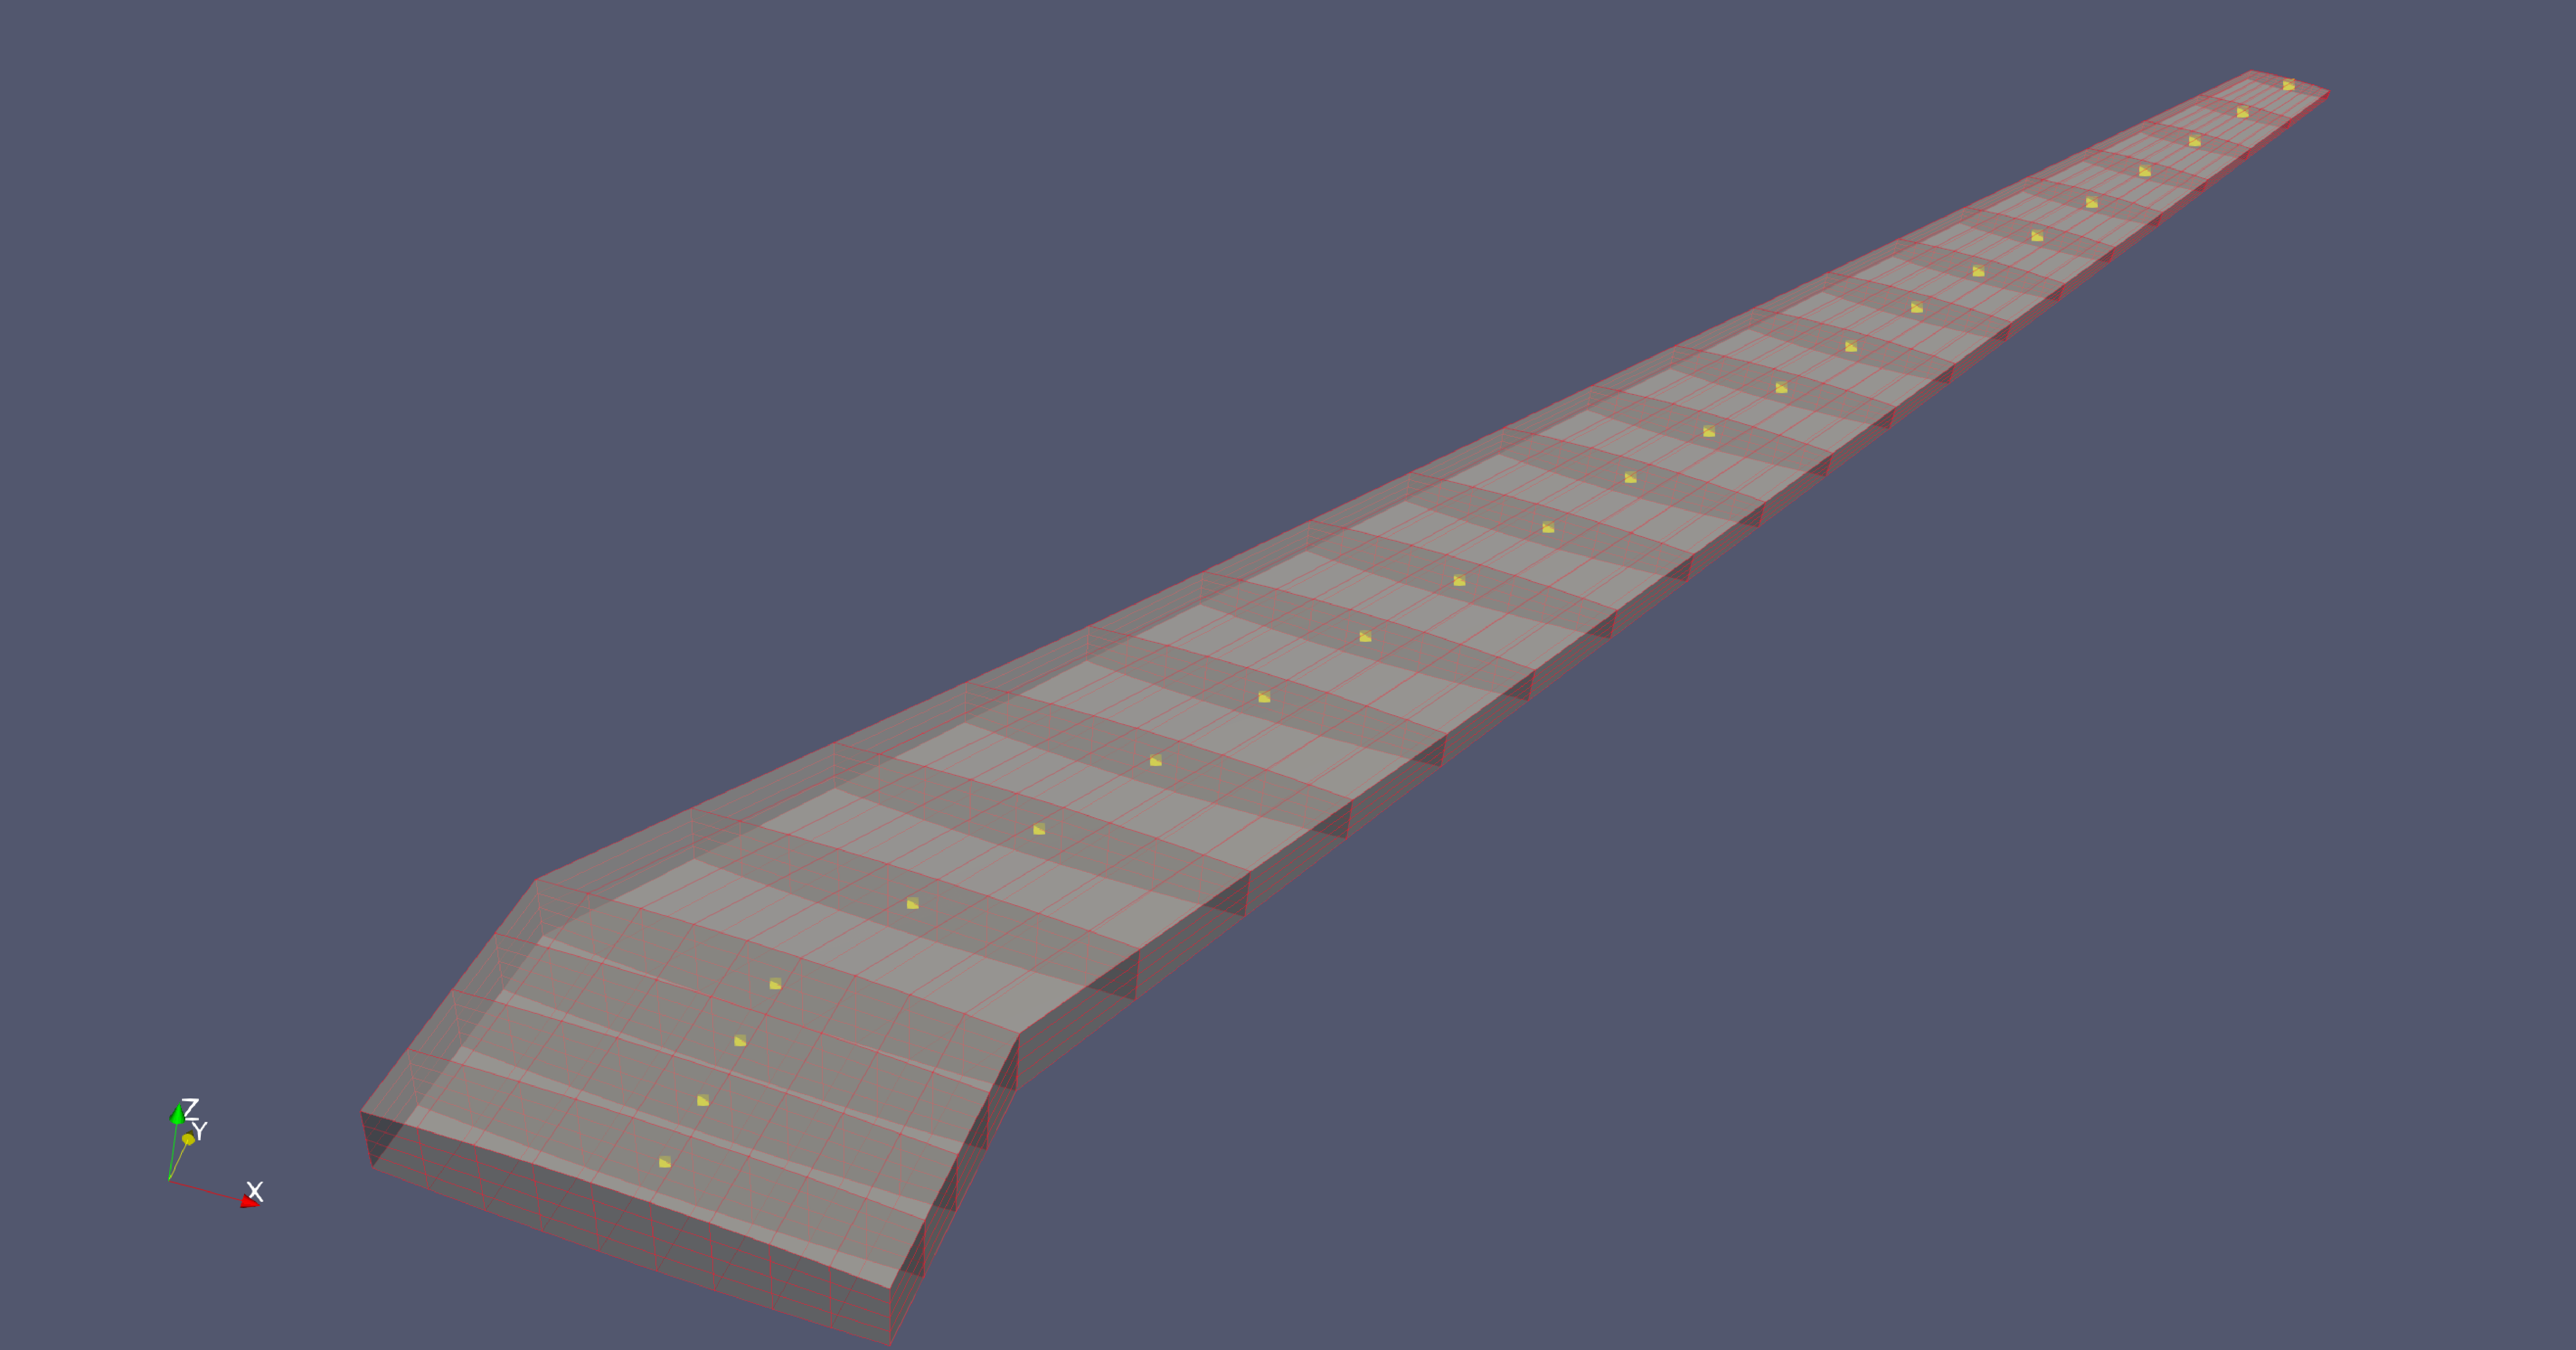
\includegraphics[width=0.495\textwidth]{./img/wingSP5}}
\subfigure[\label{fig:wing-box2}Design with rib-holes ($M_2$)]{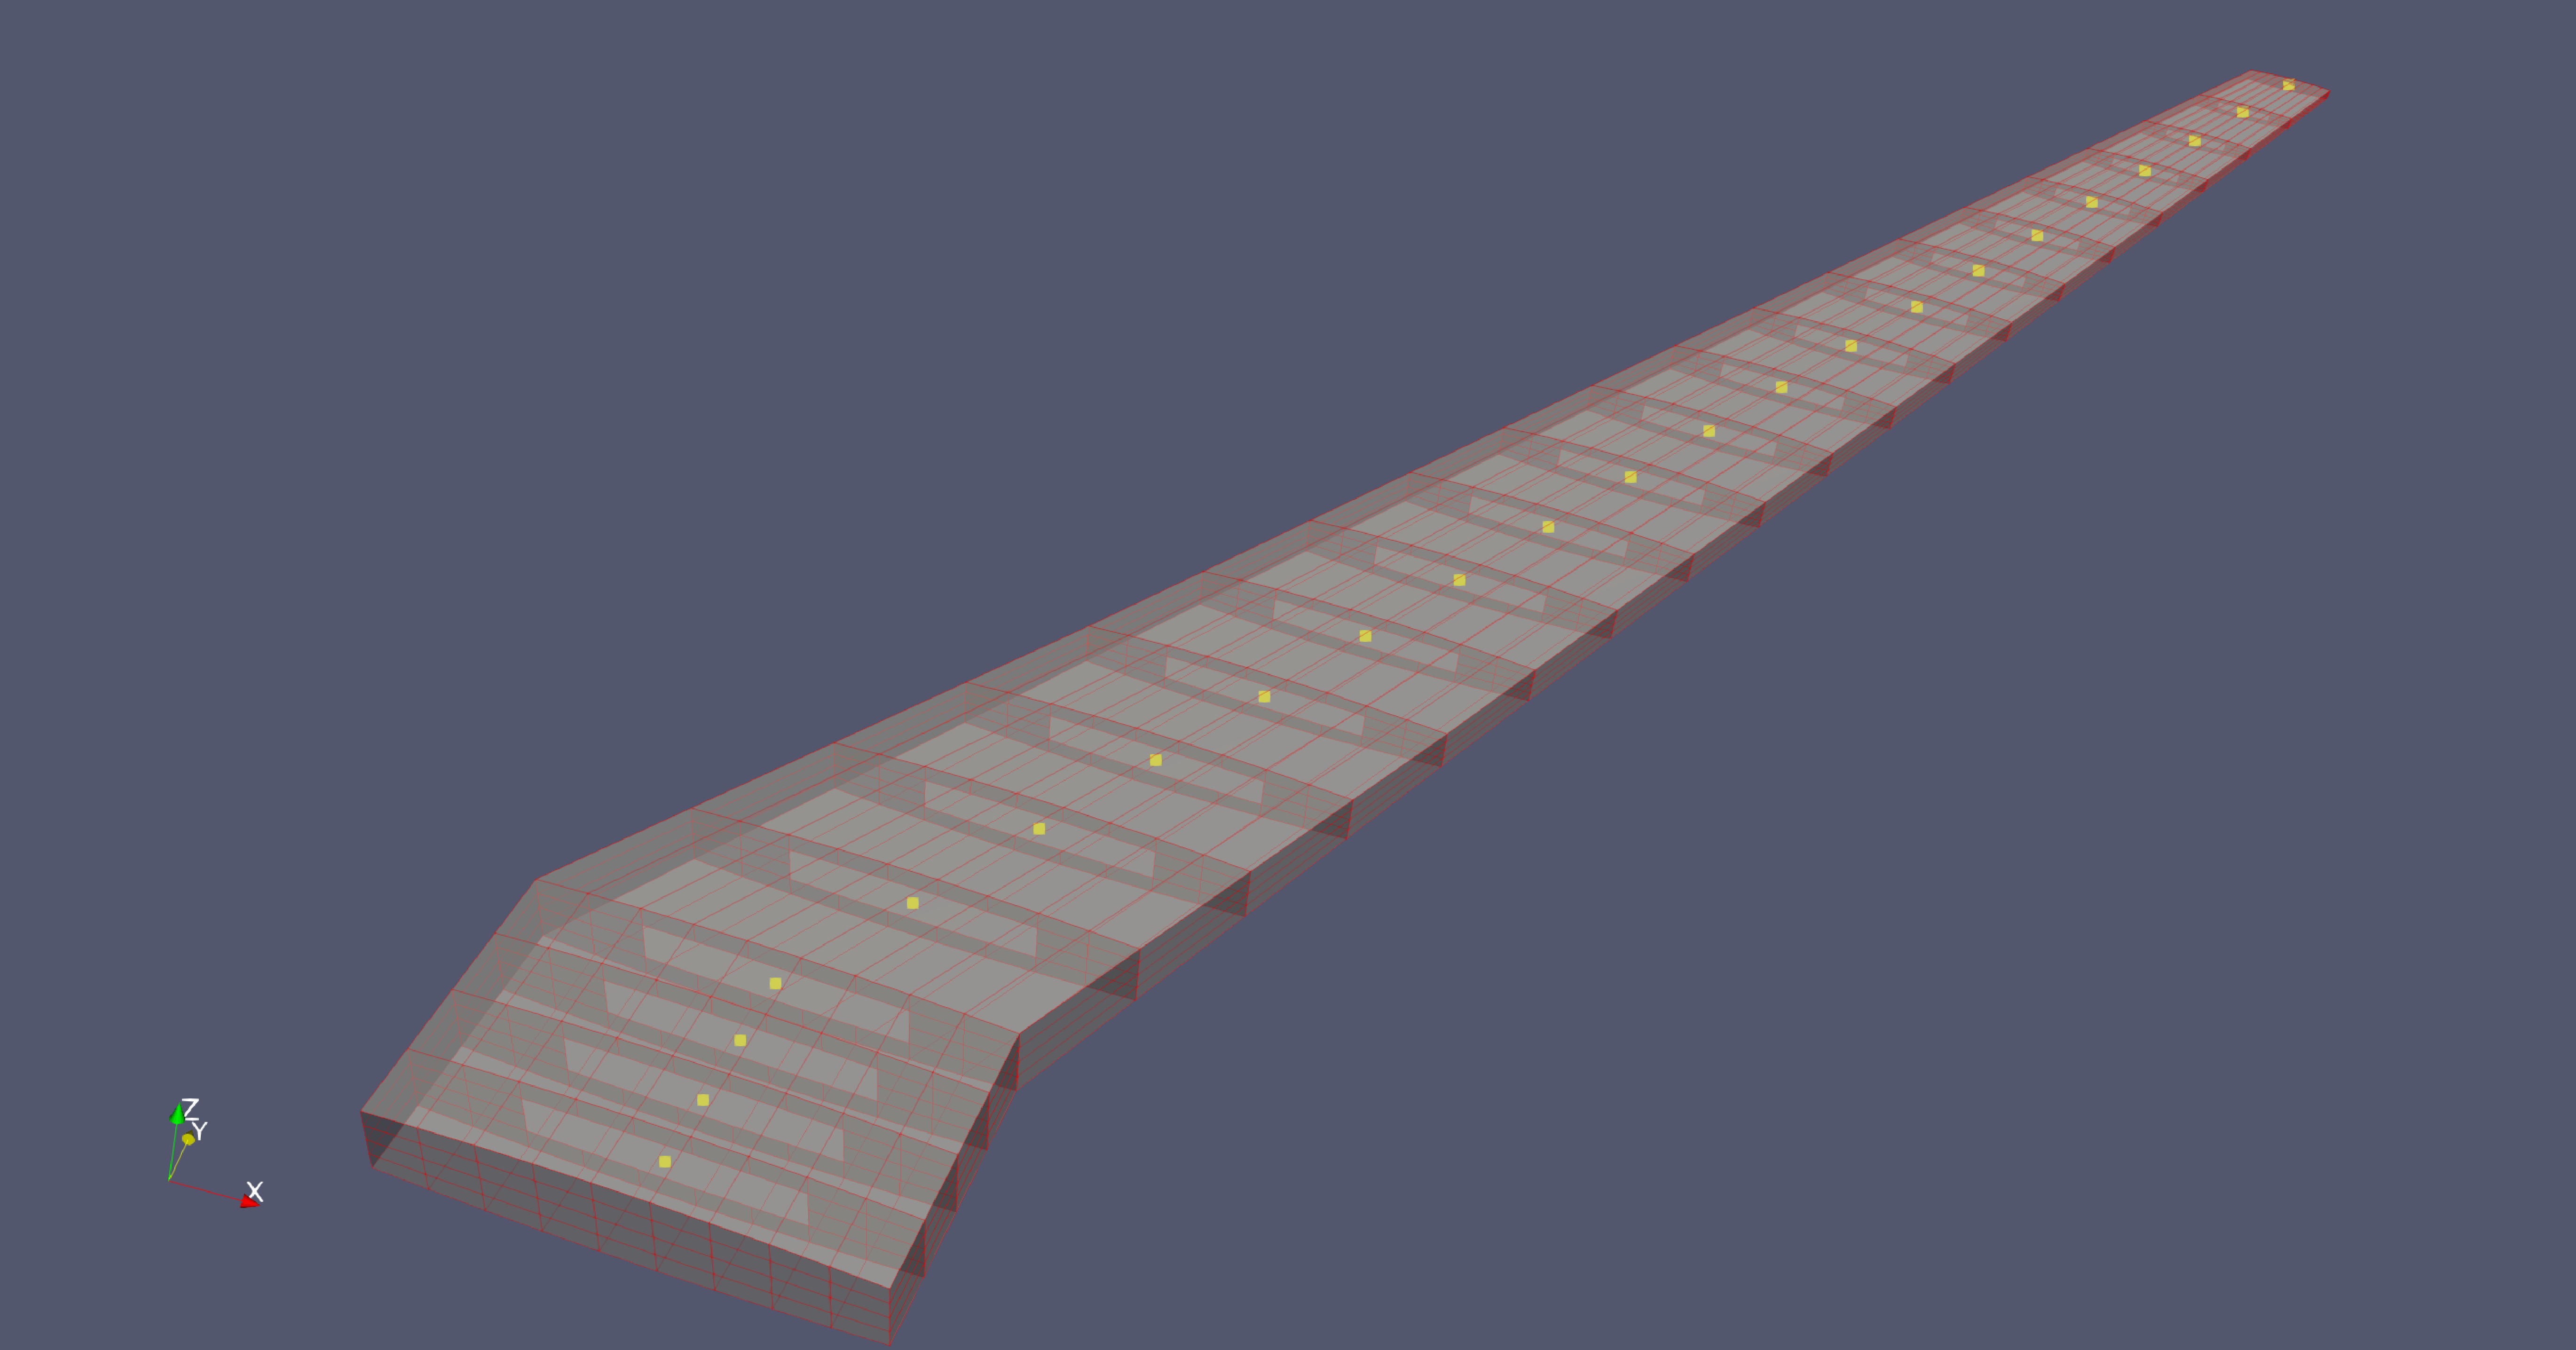
\includegraphics[width=0.495\textwidth]{./img/wingSP_ribhole5}}
\caption{Two representative wing models with the chordwise direction along the x-axis and wing-span along the y-axis. Dots indicate the condensation nodes}\label{fig:wing-box}
\end{figure}
%
Figure \ref{fig:M-relative_error} shows, for the first 32 modes on each wing, the relative error with respect to the full model in the natural frequencies predicted by the Guyan and Kidder condensations. For reference, the first natural frequency is 0.355 Hz for $M_1$ and 0.342 Hz for $M_2$, while for the 32nd mode they are 64.84 Hz and 40.90 Hz, respectively. As it can be easily seen, for the wing with the more rigid ribs, the maximum error in the Guyan condensation is just above 0.5\% and therefore this approach is sufficient to capture the higher frequencies. For wing $M_2$, where more complex cross-sectional behaviour occurs, the iterative method is necessary to capture the higher-order frequencies.

The density map of the stiffness matrices of the models gives some insight into the condensation process. Fig. \ref{fig:Ka_matrix} shows the condensed stiffness matrix for both the rigid ($M_1$) and flexible ($M_2$) wings, using Kidder condensation. 

\begin{figure}[h!]
\centering
\subfigure[\label{fig:Ka_matrix1} $M_1$ wing]{\includegraphics[width=0.42\textwidth]{./img/Ka}}
\subfigure[\label{fig:Ka_matrix2} $M_2$ wing]{\includegraphics[width=0.42\textwidth]{./img/Ki_ribhole}}
\caption{Density map of the condensed stiffness matrix in both wing models}\label{fig:Ka_matrix}
\end{figure}
For $M_1$ there are virtually no changes in the updated process of the Kidder reduction and this density map is identical to the  one obtained from Guyan reduction. The density map of the wing with flexible ribs, Fig. \ref{fig:Ka_matrix2}, shows a much denser condensed matrix, which suggests that the iterative methods pack more information into the matrix to preserve the fidelity of the full model.
Dynamic nonlinear  simulations are carried out next and compared to MSC Nastran linear and nonlinear analysis (SOL 109 and 400, respectively) on the full FE model. A force is applied at the wing tip with a triangular loading profile given as  
\begin{equation}\label{eq:loading}
  f(a,b,c) =
    \begin{cases}
      a+\frac{1-a}{b}t & \text{if $t \leq b$}\\
     1-\frac{1}{b+c}t & \text{if $b<t \leq b+c$}\\
      0 & \text{otherwise}
    \end{cases}       
\end{equation}
The follower force applied to the tip of $M_1$ is a ramp, $\pmb{f}_{tip}= [-2\times 10^5,0,6\times 10^5]f(0.05,4,0.)$ and the dynamic response is presented in Fig. \ref{fig:sp_results}, where results have been normalised with the wing semi-span. As expected, linear analysis overpredicts vertical displacements and does not capture displacements in the $x$ and $y$ directions. Using Guyan condensation, which is sufficient for this wing, NMROMs were built with 15 and 50 modes and run with time-steps of $6 \times 10^{-3}$ and $3 \times 10^{-3}$ respectively. 

\begin{figure}[h!]
\centering
\includegraphics[width=0.9\textwidth]{./img/wingSP11}
\caption{Span-normalised tip displacements in the dynamic simulation of $M_1$}\label{fig:sp_results}
\end{figure}

\subsubsection{Generalised aerodynamic forces}
\label{sec:orgd7bc12a}
Figure 13 shows a subset of the GAFs for this platform up to \(\kappa = 2\) obtained with a sampling of \(\delta \kappa = 0.01\). Four
GAFs have been selected, corresponding to the first three wing bending modes and the first torsional mode, and they are
shown in that order in the figure. The same preconditioning scheme of section III has been used, namely, the best fit
to the local values of aerodynamic stiffness, mass and inertia at that limit frequency (\(\kappa = 2\)). The effect of this is to
reduce the value of the residual transfer function at the highest frequencies in the training dataset, which accelerates
the convergence of the Loewner matrix approach. Figure 13 shows the results for 12 states obtained both with and
without the polynomial preconditioning. As it can be clearly seen, introducing the preconditioning vastly improves the
accuracy of the LTI model of a given size. The Loewner interpolant solution algorithm used in this work does not
enforce stability and in this case all models are unstable. 
\begin{center}
\includegraphics[width=.9\linewidth]{./img/dlm_precond.pdf}
\end{center}
\subsubsection{Preliminary aeroelastic assessment}
\label{sec:org7ca754f}

\subsection{Dynamic loads on the XRF1 aircraft}

The studies presented in this chapter are based on a reference configuration developed to industry standards by Airbus as part of the eXternal Research Forum (XRF), from which the aircraft takes its name, XRF1. The aircraft represents a long-range wide-body transport airplane  and has been used as a research platform for collaboration between the company, universities and research institutions \cite{Klimmek2019}. The original model has been modified for this work and contains a wing tip extension that makes the overall aspect ratio of the wing slightly higher and can be used as an aeroelastic hinge device for load alleviation, although for most of this  work  the whole mechanism remains attached and only at the end it is released to carry out a preliminary study of a foldable wings concept. %The baseline configuration is called XRF1-IC (for Imperial College). 
Fig. \ref{fig8:xrf1-model} shows the full aeroelastic model split up into the structural, mass and aerodynamic components. The FE model contains a total of around 177400 nodes, which are condensed into 176 active nodes along the reference load axes through interpolation elements (RBE3s with the UM option as described in \cite{Klimmek2014}). A Guyan or static condensation approach is used for the reduction, which is equivalent to a dynamic condensation when the mass model is given as discrete elements at the condensation points, as is the case here -- for distributed mass elements other dynamic condensation techniques might give better results as shown above. Among the FE elements conforming the model there are around $\sim 500$ spring, or 0-dimension elements; $\sim 57,000$ beam elements, $\sim 55,500$ CQUAD4 shell elements, $\sim 3,800$ CTRIA3 shell elements; and $\sim 800$ rigid elements. As for the mass configurations, the one utilised in this study is the estimated cruise reference mass, which amounts to a total of $\sim 188,500$ kg. The aerodynamic model contains $\sim 1,500$ aerodynamic panels.

\begin{figure}[th!]
\centering
\includegraphics[width=1.\textwidth]{./img/xrf1-model.pdf}
\caption{Modified XRF1 aeroelastic subcomponents }\label{fig8:xrf1-model}
\end{figure}
There are other methods for working with these large models in an efficient manner and incorporating geometrically nonlinear effects, for instance deriving equivalent stick models by imposing unitary loads \cite{AElsayed2009} in the original model and finding the beams that better match the linear response to these loadings. Another alternative is creating a data base with nonlinear static computations of the full model, which is used for system identification of the properties of a reduced order model of the structure \cite{Medeiros2019}.
 However, one of the major advantages of the current methodology is that prior nonlinear calculations are not required to find the ROM, nor equivalent designs built that could lose some details of the original model. The only operation is a condensation step where the full aircraft model is reduced into the major load-paths. This is already a common practice in the aeroelastic industrial environment and the reduced model of the XRF1 was also provided. The strength of the approach can be seen by looking at the natural f

The introduction and verification of compressible effects was performed replicating the exercise in Fig. \ref{fig:gust1-1235-1_001} with gust number 3 but including results from a simulation at 0.81 Mach number. A very good match is again found and it is shown in Fig. \ref{fig:gust131_001-081Ma} that the compressible effects act to increase the overall loading on the wings.  

Similar to the previous exercise, comparisons are presented for large displacements  by setting $w_{g0} = 2$ for gust 3 at $M_\infty = 0$ and $M_\infty = 0.81$. If compressible and geometrically nonlinear effects are analysed separately, it may be said that the former has a more important effect in the $z$-component of the displacements, i.e. in the module of the aerodynamic loading; while the latter changes the response in $x$ and $y$ components more significantly, i.e. in the direction of the loading. It should also be noted that the dynamics excited by these type of disturbances, mostly driven by the first bending modes, are not very complex and very different effects are expected in more involved exercises as it could be the combination of dynamic manoeuvres with random atmospheric disturbances.  In this initial phase, however, the primary goal is to demonstrate that linear results from commercial loads packages are replicated for small deflections and that geometric nonlinear effects are seamlessly incorporated when significant deflections take place. Moreover, the approach has to work with the full FE models used in load analysis and take into account compressible effects. These characteristics combined are not met by current state-of-the-art methods.

\begin{figure}[h!]
\centering
\includegraphics[width=0.95\textwidth]{./img/gust131_2-081Ma.pdf}
\caption{Wing-tip dynamic response for high intensity gust at Mach 0-0.81}\label{fig:gust131_2-081Ma}
\end{figure}
\newpage
Next we are carrying out simulations with gust shapes (b) and (c) in Fig. \ref{fig8:gust_shapes}. The gust length is 67 m.,  air density of 0.778 kg/m$^3$ and speed of 185 m/s, and 0 Mach number. The gust intensity is  $w_{g0} = 7$ in the asymmetric gust and  $w_{g0} = 10$ in the DARPA gust in order to achieve maximum wing tip deformations within 27-33 \% in both cases. Instead of plotting those wing displacements, the comparison of moments at the wing root is shown in Fig. \ref{fig8:MxMy} as a more relevant metric for design. The plot  corresponds to the first second of simulation when the gust acts and maximum loads appear in the structure. 

\begin{figure}[ht!]
\centering
\subfigure[Asymmetric gust shape]{\includegraphics[width=0.481\textwidth]{./img/MxMy_antisym211b.pdf}}
\subfigure[Darpa gust shape]{\includegraphics[width=0.51\textwidth]{./img/MxMy_darpa211b.pdf}}
\caption{Wing root moments evolution due to gust disturbance}\label{fig8:MxMy}
\end{figure}
%It is worth remarking the moments are are given in a local reference system such  that $M_x$ is the moment along the wing reference load path, producing torsion of the wing, and $M_x$ perpendicular to it and and giving rise to out-of-plane bending deformations. 
Linear and nonlinear comparisons, both carried out within FEM$_4$INAS framework, show that linear analysis may produce some  non-conservative critical loads, which could lead to failure, or overly conservative in other design points, which could mean heavier than necessary structures. This is a known effect in the literature of high aspect ratio, long endurance aircraft \cite{Palacios2014}, although it has been rarely explored on large transport aircraft. The next step in the analysis would be integrating the approach into an automatic process such that thousands of simulations can be run automatically  in parallel, maximum loads extracted and the final load envelopes built comparing the linear versus nonlinear assumptions across all flight conditions. Yet we are showing the methods can deal with industrial models, not trying to solve  the entire industrial process. 
\\

\section{Summary}
\label{sec:summary}


\bibliographystyle{abbrv}
\bibliography{/home/ac5015/Documents/Engineering.bib}

\end{document}
%%% Local Variables:
%%%## reftex-default-bibliography: ("/home/acea/Documents/Engineering.bib")
%%% reftex-default-bibliography: ("/home/ac5015/Documents/Engineering.bib")
%%% TeX-command-extra-options: "--synctex=1"
%%% TeX-master: t
%%% End: